%%%%%%%%%%%%%%%%%%%%%%%%%%%%%%%%%%%%%%%%%%%%%%%%%%%%%%%%
%GRASS PROMOTION FLYER                                 %
%(c) 2007 GRASS PROMOTION TEAM                         %
%GNU Free Documentation License                        %
%Version 1.2                                           %
%Needs leaflet.cls				       %
%www.ctan.org/tex-archive/macros/latex/contrib/leaflet/%
%%%%%%%%%%%%%%%%%%%%%%%%%%%%%%%%%%%%%%%%%%%%%%%%%%%%%%%%

%Sometimes printing engines need the 2nd side upside down
%in this case, use tumble (which is default) instead of notumble
%If this causes problems, use notumble
%If you need a foldmark, delete nofoldmark
\documentclass[notumble,a4paper,10pt,nofoldmark]{leaflet}
\usepackage{helvet,courier,xcolor}

% Set Helvetica as the default font
\renewcommand*\familydefault\sfdefault
% Let LaTeX knows that pictures are found in ./pix
\graphicspath{{pix/}}

% Setting up things for the captions
\usepackage{caption}[2004/07/16]
\captionsetup{%
  font={small,it},%
  labelformat=empty,% Leaves out label: ``Figure 1''
  labelsep=none,%
  aboveskip=0pt%
}
% Defining a new 'figure' environment for the document
\newenvironment{myfig}[1][0pt plus 1.5ex minus .5ex]{\par\vspace*{#1}\begin{minipage}{\textwidth}\centering}{\end{minipage}}

% Defining the GRASS homepage
\newcommand{\GRASSurl}{\url{http://grass.itc.it}}

% Define a color for the URIs
\definecolor{darkblue}{RGB}{0,0,88}

\usepackage{hyperref}
% Setting up some document info
\hypersetup{%
  colorlinks=true,%
  urlcolor=darkblue,% Redefine this color to change URIs color
  pdfauthor={The GRASS Community},%
  pdftitle={GRASS GIS: Efficiency through Freedom \& Transparency},%
  pdfsubject={GRASS Promotion Flyer},%
  breaklinks=true,%
  plainpages=false%
}

% Title page stuff
\title{\textbf{\huge GRASS GIS}\\%
\textsl{Efficiency through Freedom \& Transparency}}
\author{The GRASS Community}
\date{
\includegraphics[width=\textwidth]{grasslogo_vector}\\[2ex]
\large\GRASSurl}

\begin{document}

\maketitle
\thispagestyle{empty}% Necessary to leave out the page number on the first page

\newpage

\section{What is GRASS}

GRASS (Geographic Resources Analysis Support System) is a free and Open Source Software for performing spatial analysis. It consists of more than 350 modules for processing vector (2D/3D), raster and voxel data. Many interfaces to other programs in related domains like geostatistics, databases, mapserver and even other GIS software exist. It is the largest Open Source GIS. It can serve as a Desktop GIS and as the backbone of a complete GIS Infrastructure.

\section{Where is GRASS used}

GRASS is used in scientific applications, commercial settings and by public authorities all over the world. GRASS has shown strong potential for solving geospatial problems in numerous situations world-wide.

\section{History}

GRASS was originally developed in the beginning of the 1980's by the US Army Construction Engineering Research Laboratories (USA-CERL) and was published as public domain software. When the USA-CERL withdrew from GRASS development, an international developer team took over this work. Since 1999, GRASS has been published as free software under the terms of the GNU General Public Licence.
\begin{myfig}[1.5ex]
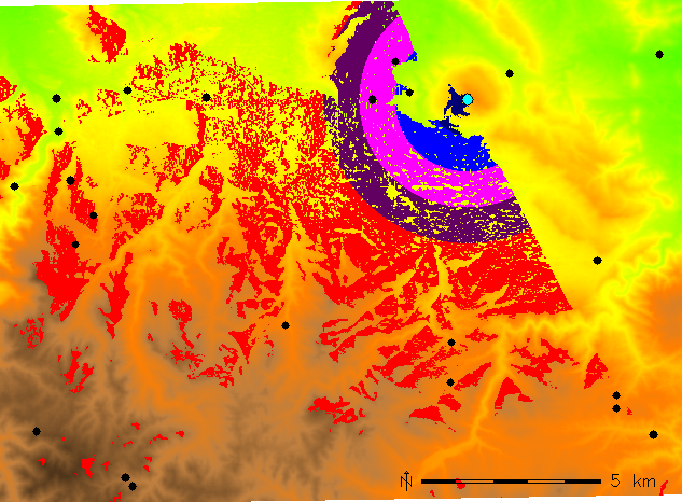
\includegraphics[width=0.7\textwidth]{visibility}
\captionof{figure}{Viewshed analysis performed with GRASS}
\end{myfig}

\section{Open Source Philosophy}

The Open Source philosophy provides the user the ability to see the source code and structure of the program which offers a great transparency. Users can extend the program for their own needs. Immediate souce code peer review increases the quality. With the help of the extension manager new modules can be created without GRASS package source code.

\section{Technical Data Sheet}

\subsection{License}

GNU General Public License (Free Software Foundation)

\subsection{Supported platforms}

GRASS runs on nearly all platforms. It supports GNU/Linux, Posix compliant Unix Systems, MS-Windows and MacOS X.

\subsection{Design}

\begin{itemize}
\item Modular
\item Consists of more than 350 modules
\end{itemize}

\subsection{Programming Languages}

\begin{itemize}
\item ANSI C
\item GRASS- SWIG interface
\item Python for WebGIS applications
\item Java Version: JGRASS
\end{itemize}

\subsection{Data Management Capabilities}

\begin{itemize}
\item Raster / Vector / Voxel data processing
\item 2D / 3D Raster / Vector modelling
\item Image manipulation
\item Vector topology / Network analysis
\item Geostatistics (Interface to R)
\end{itemize}

\begin{myfig}[1ex]
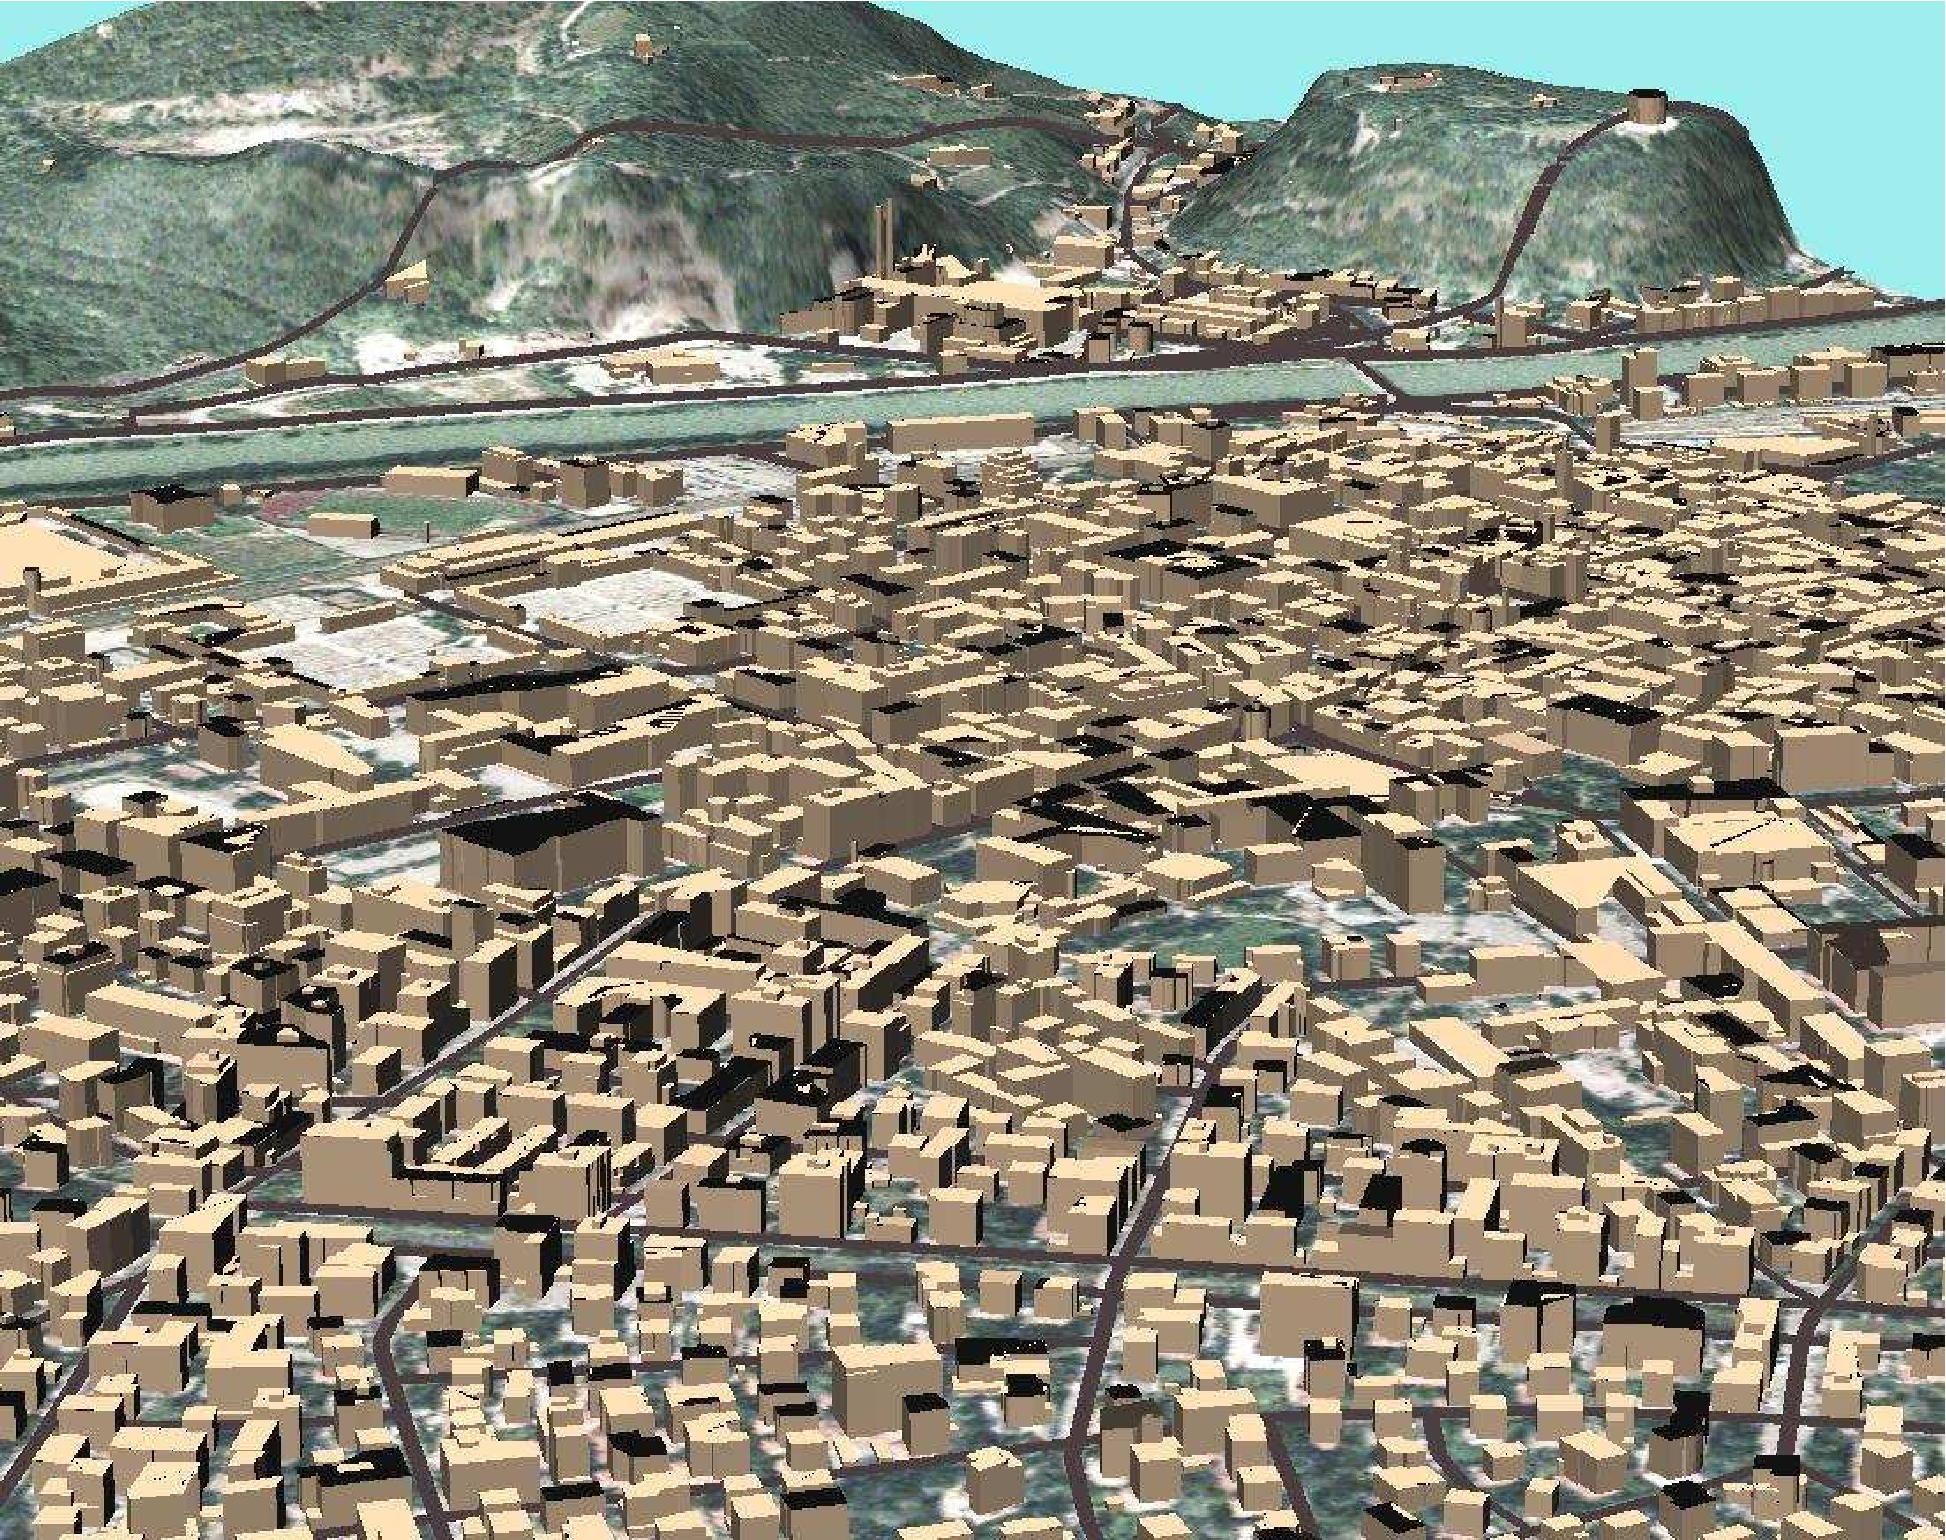
\includegraphics[width=0.7\textwidth]{trento3d}
\captionof{figure}{A flyby of the city of Trento, Italy}
\end{myfig}

\section{Supported File Formats}

GRASS supports nearly all common GIS file formats through the use of the GDAL/OGR library. In addition it supports the Open GIS Consortium's Simple Features.

\subsection{Vector File formats}
ASCII, ARC/INFO ungenerate, ARC/INFO E00, Arc\-View SHAPE, BIL, DLG (U.S.), DXF, DXF3D, GMT, GPS-ASCII USGS-DEM, IDRISI, MOSS, MapInfo MIF, TIGER, VRML, \dots

\subsection{Raster File Formats}
ASCII, ARC/GRID, E00, GIF, GMT, TIF, PNG, Vis5D, SURFER (.grd),\dots
\begin{myfig}
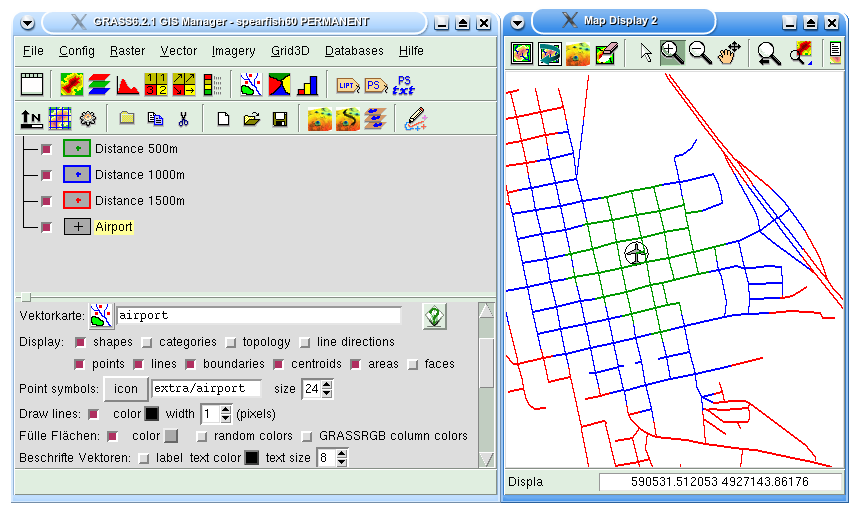
\includegraphics[width=0.7\textwidth]{isodist}
\captionof{figure}{Default GUI configuration showing GRASS  network analysis capabilites}
\end{myfig}

\subsection{Image File Formats}

CEOS (SAR, SRTM, LANDSAT7 etc.), ERDAS LAN / IMG, HDF, LANDSAT TM/MSS, NHAP aerial photos, SAR, SPOT, \dots
\begin{myfig}[1.5ex]
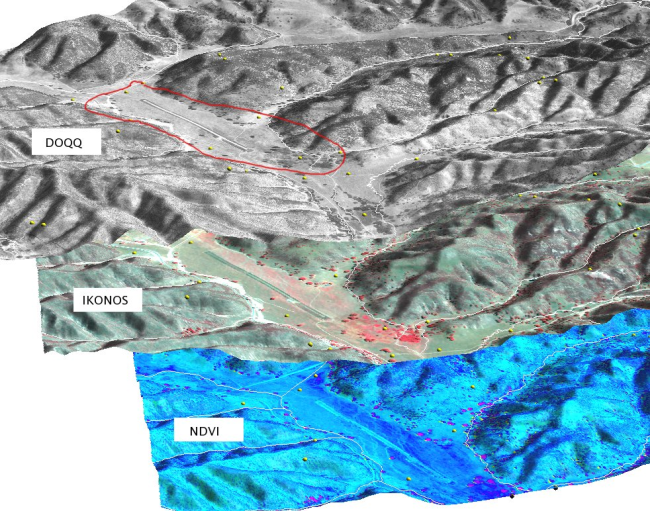
\includegraphics[width=0.7\textwidth]{ndvi}
\captionof{figure}{Image processing capabilities of GRASS}
\end{myfig}

\subsection{Database support}

\begin{itemize}
\item PostgreSQL / PostGIS
\item MySQL
\item SQLite
\item ODBC
\item DBF
\end{itemize}

\subsection{Output}

\begin{itemize}
\item Modules for creating maps
\item NVIZ for visualization of 2.5D and 3D data (creation of animations \& flybys)
%\item{GMT export}
%item{VRML}
\item VTK, POVray
\item WebGIS via Mapserver, Python, etc.
\end{itemize}

\subsection{Interoperability to other GIS- related Software}

\begin{itemize}
\item Quantum GIS (Free Geodata Viewer and more)
\item R- Language (Statistics)
\item Gstat (Geostatistics)
\item UMN Mapserver (Webmapping)
\end{itemize}

\section{Where to find more information}

\begin{itemize}
%\begin{flushleft}
\item{Project Website: \\\GRASSurl}
\item{GRASS Wiki: \\\url{http://grass.gdf.hannover.de/wiki}}
\item{GRASS Promotion Team: \\\url{malte@perlomat.de}}
\item{GRASS mailing lists: \\\url{http://grass.itc.it/community/support.php}}
%\end{flushleft}
\end{itemize}

\vfill
\section{OSGeo}

GRASS is a founding project of the Open Source Geospatial Foundation which has the aim to create high quality open source geospatial software. For further information visit the OSGeo homepage:
\begin{center}

\includegraphics[width=0.8\textwidth]{OSGeo_CMYK}\\
\url{http://www.osgeo.org}
\end{center}

\end{document}
